%*****************************************
\chapter{Implementation}
\label{ch:implementation}
%*****************************************

%\hint{This chapter should describe the details of the implementation addressing the following questions: \\ \\
%1. What are the design decisions made? \\
%2. What is the environment the approach is developed in? \\
%3. How are components mapped to classes of the source code? \\
%4. How do the components interact with each other?  \\
%5. What are limitations of the implementation? \\ \\
%The section should have a length of about five pages.}

%\section{Design Decisions}
%\textbf{Tensorflow 2.0} is used as the framework for all experiments presented in this thesis. It %enables software development on a high level of abstraction while ensuring code performance. Because some
%procedures are not naturally compatible with the implementation of Tensorflow 2.0  this thesis needs to %employ a few workarounds. Notably pruned weights are not removed from the network but rather set to %zero each time a layer is evaluated. As such they do not affect the predictions but are influenced by %backpropagation. \textit{The effect on the presented experiments is unclear to me.}
%
%\subsection{Missing Parameters}
%Through the related work referenced in this thesis specifications of any one model where incomplete. %The following subsection aims to explain how the parameters were inferred or chosen. 
%\begin{itemize}
%	\item Activation function for most layers
%	\item Activation function for output layers
%	\item Dropout rate
%	\item padding in CNNs
%	\item ...
%\end{itemize}

\section{Representation in the Framework}
\begin{figure}
	\begin{minipage}{0.45\textwidth}
		\centering
		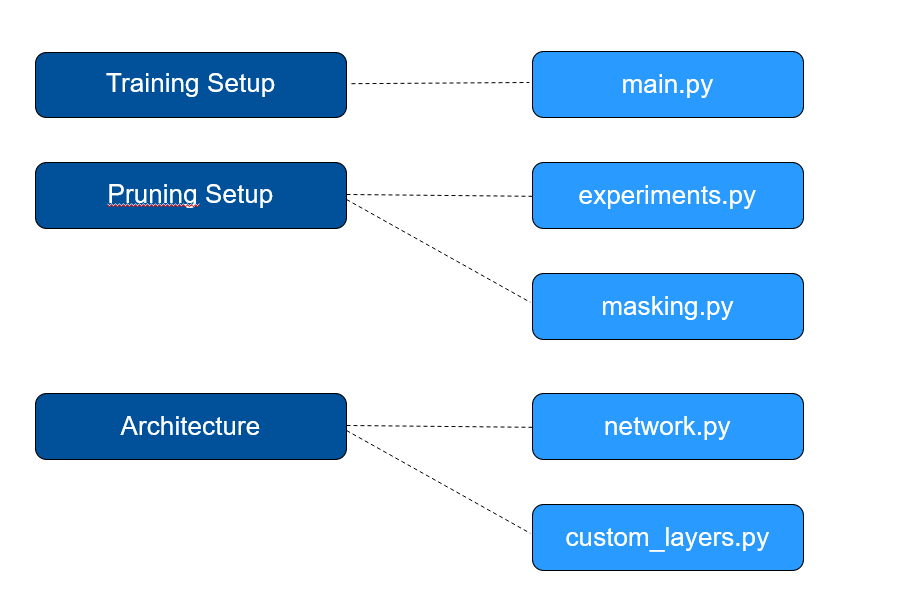
\includegraphics[width=200px]{gfx/chp_5_setups.png}
		\caption{Representation of the main components in the framework}
		\label{fig:Setup Representation}
	\end{minipage}\hfill
	\begin{minipage}{0.45\textwidth}
		\centering
		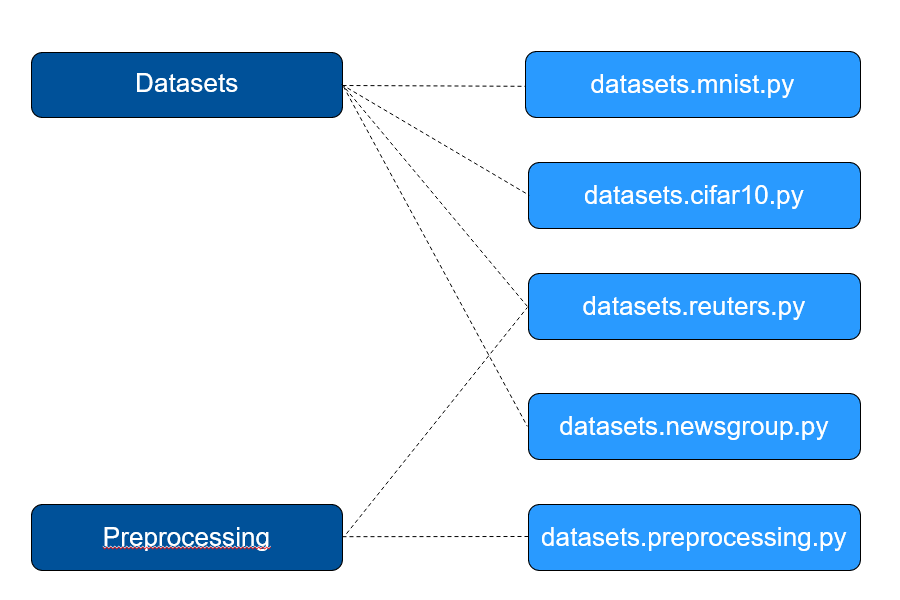
\includegraphics[width=200px]{gfx/chp_5_datasets.png}
		\caption{project architecture}
		\label{fig:Dataset Representation}
	\end{minipage}
\end{figure}
%\begin{figure}[h]
%	\centering
%	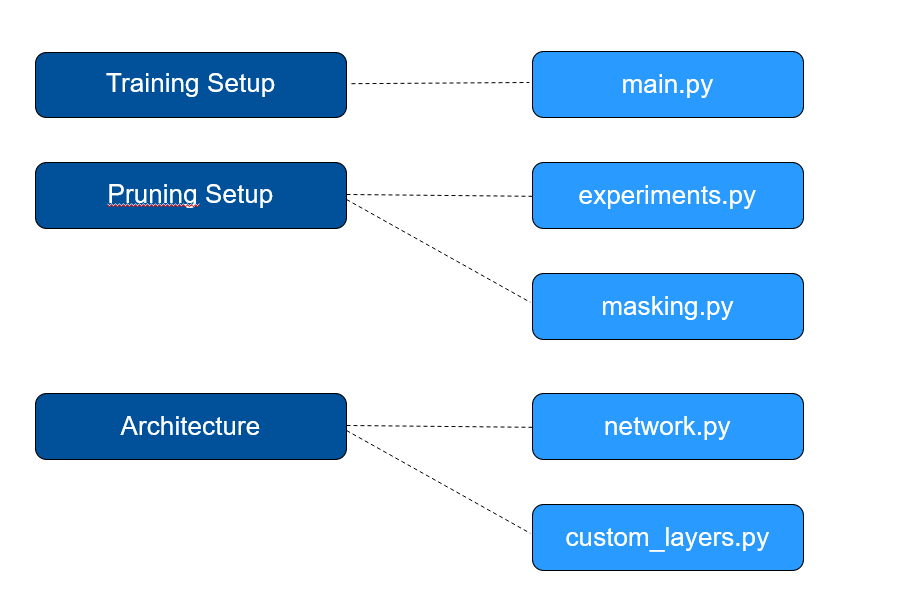
\includegraphics[width=450px]{gfx/chp_5_setups.png}
%	\caption{Representation of the main components in the framework}
%	\label{fig:Setup Representation}
%\end{figure}
%\begin{figure}[h]
%	\centering
%	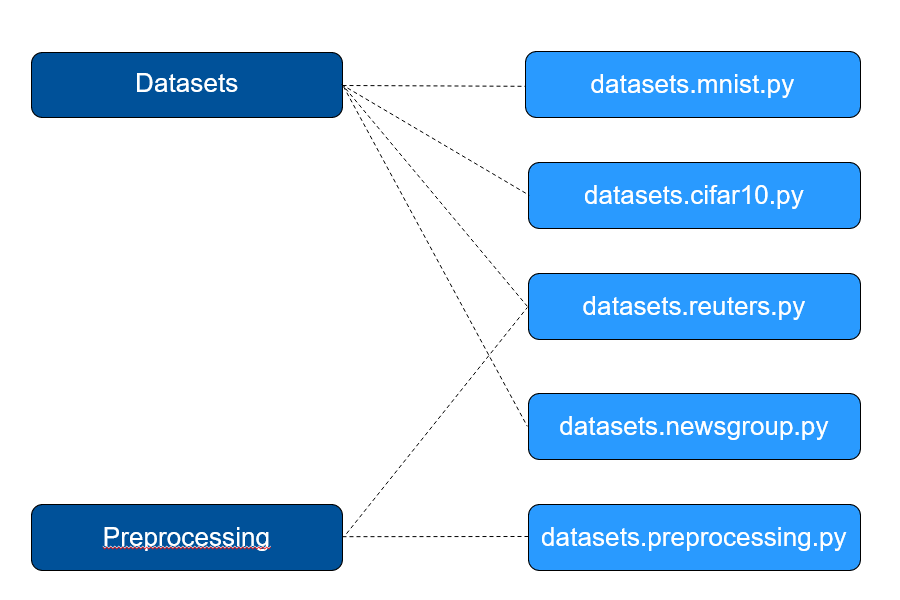
\includegraphics[width=450px]{gfx/chp_5_datasets.png}
%	\caption{project architecture}
%	\label{fig:Dataset Representation}
%\end{figure}

\section{Framework Internals}
\subsection{Control Flow and Hierarchy of Abstractions}

\begin{figure}
	\centering
	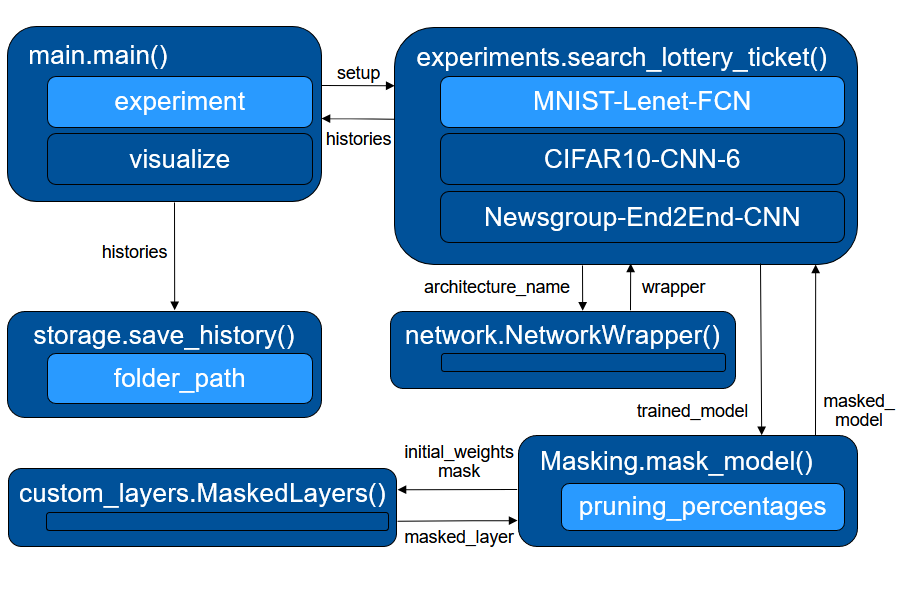
\includegraphics[width=450px]{gfx/chp_5_control_flow.png}
	\caption{Scheme of the framework during an example experiment}
	\label{fig:Example Control Flow}
\end{figure}
\subsection{Backend}

\section{Limitations}